%---------------
%╔═╗╔═╗╔╦╗╦ ╦╔═╗
%╚═╗║╣  ║ ║ ║╠═╝
%╚═╝╚═╝ ╩ ╚═╝╩  
%---------------

% language setup
\newcommand{\docLanguage}{ngerman}
%\newcommand{\docLanguage}{english}

% DOCUMENT SETUP
\documentclass[12pt, oneside, a4paper, \docLanguage]{report}
\usepackage[left=3cm, 
			right=2.5cm, 
			top=2.5cm, 
			bottom=2.5cm, 
			includehead, 
			includefoot]{geometry}

% line spacing
\usepackage{setspace}
\setstretch{1,25} % 15/12 --> 1.25

% encoding setup
% T1 font encoding for languages that use a latin alphabet
\usepackage[T1]{fontenc} 

% enhanced input encoding handling - utf8 for äÄüÜöÖß...
\usepackage[utf8]{inputenc}

%de­fines Adobe Times Ro­man as de­fault text font
\usepackage{mathptmx}
\usepackage{times} % needed for acronym package

%PDF linking package
\usepackage[hidelinks]{hyperref}


% Language Setup
\usepackage[\docLanguage]{babel}
% after babel - set chapter string
\AtBeginDocument{\renewcommand{\chaptername}{}}

% language specific bibliography style
\usepackage[numbers, square]{natbib}
%\setcitestyle{square,aysep={},yysep={;}}
\usepackage[fixlanguage]{babelbib}
\selectbiblanguage{\docLanguage}
% bliographystyle setup
% babel specific: babplain, babplai3, babalpha, babunsrt, bababbrv, bababbr3
\bibliographystyle{babunsrt}


% enumeration
\usepackage{enumitem}
% tabular extension tabularx
\usepackage{tabularx}

% math packages
\usepackage{amsmath}
\usepackage{nicefrac}
\usepackage{amsthm}
\usepackage{amsbsy}
\usepackage{amssymb}
\usepackage{amsfonts}
%\usepackage{MnSymbol}


%special characters
\usepackage{amssymb}
\usepackage{upgreek,textgreek}

% acronym package
\usepackage[printonlyused, footnote]{acronym}

% breakable text in \seqsplit{}
\usepackage{seqsplit}

% \textmu
\usepackage{textcomp}

% package provides a way to compile sections of a document using the same preamble as the main document
\usepackage{subfiles}

% driver-independent color extension - used by listings,tabularx
\usepackage[usenames,dvipsnames,table,xcdraw]{xcolor}

% -- SYNTAX HIGHLIGHTING --
\usepackage{listings}
%% bash command line Syntax Highlighting
\lstdefinestyle{BASH_CMD}{ 
  columns=fullflexible,            % copy pasteable listings
  language=bash,
  basicstyle=\small\sffamily,
  basicstyle   = \small \ttfamily,
  keywordstyle = [1]\small \ttfamily,
  keywordstyle = [2]\small \ttfamily,
  commentstyle = \small \ttfamily,
  numbers=none,
  captionpos=b, 
  breaklines=true,
  numberstyle=\tiny,
  numbersep=3pt,
  frame=tlrb,
  columns=fullflexible,
  backgroundcolor=\color{white!20},
  linewidth=\linewidth,
  literate=                        % replace in code
     {Ö}{{\"O}}1 
     {Ä}{{\"A}}1 
     {Ü}{{\"U}}1 
     {ß}{{\ss}}2 
     {ü}{{\"u}}1 
     {ä}{{\"a}}1 
     {ö}{{\"o}}1 
     {â}{{\^{a}}}1 
     {Â}{{\^{A}}}1 
     {ç}{{\c{c}}}1 
     {Ç}{{\c{C}}}1 
     {ğ}{{\u{g}}}1 
     {Ğ}{{\u{G}}}1 
     {ı}{{\i}}1 
     {İ}{{\.{I}}}1 
     {ş}{{\c{s}}}1 
     {Ş}{{\c{S}}}1 
}
 % adds style BASH_CMD
%% Matlab Syntax Highlighting
\colorlet{keyword}{blue!100!black!80}
\colorlet{STD}{Lavender}
\colorlet{comment}{green!90!black!90}
\definecolor{mygreen}{rgb}{0,0.6,0}
\definecolor{mygray}{rgb}{0.5,0.5,0.5}
\definecolor{mymauve}{rgb}{0.58,0,0.82}


\lstdefinestyle{BASH_SCRIPT}{ 
  language     = bash,
  basicstyle   = \footnotesize \ttfamily,
  keywordstyle = [1]\color{keyword}\bfseries,
  keywordstyle = [2]\color{STD}\bfseries,
  commentstyle = \color{mygreen}\itshape,
  backgroundcolor=\color{white},   % choose the background color; you must add \usepackage{color} 
  columns=fullflexible,            % copy pasteable listings
                                   % or \usepackage{xcolor}
  basicstyle=\footnotesize,        % the size of the fonts that are used for the code
  breakatwhitespace=false,         % sets if automatic breaks should only happen at whitespace
  breaklines=true,                 % sets automatic line breaking
  captionpos=b,                    % sets the caption-position to bottom
  extendedchars=true,              % lets you use non-ASCII characters; for 8-bits encodings only,
                                   % does not work with UTF-8
  frame=single,                    % adds a frame around the code
  keepspaces=true,                 % keeps spaces in text, useful for keeping indentation of code
                                   % (possibly needs columns=flexible)
  numbers=left,                    % where to put the line-numbers; possible values are 
                                   % (none, left, right)
  numbersep=5pt,                   % how far the line-numbers are from the code
  numberstyle=\tiny\color{mygray}, % the style that is used for the line-numbers
  rulecolor=\color{black},         % if not set, the frame-color may be changed on line-breaks
                                   % within not-black text (e.g. comments (green here))
  showspaces=false,                % show spaces everywhere adding particular underscores; it
  	                               % overrides 'showstringspaces'
  showstringspaces=false,          % underline spaces within strings only
  showtabs=false,                  % show tabs within strings adding particular underscores
  stepnumber=1,                    % the step between two line-numbers. If it's 1, each line 
                                   % will be numbered
  stringstyle=\color{mymauve},     % string literal style
  tabsize=2,                       % sets default tabsize to 2 spaces
  title=\lstname,                  % set title name
  literate=                        % replace in code
     {Ö}{{\"O}}1 
     {Ä}{{\"A}}1 
     {Ü}{{\"U}}1 
     {ß}{{\ss}}2 
     {ü}{{\"u}}1 
     {ä}{{\"a}}1 
     {ö}{{\"o}}1 
     {â}{{\^{a}}}1 
     {Â}{{\^{A}}}1 
     {ç}{{\c{c}}}1 
     {Ç}{{\c{C}}}1 
     {ğ}{{\u{g}}}1 
     {Ğ}{{\u{G}}}1 
     {ı}{{\i}}1 
     {İ}{{\.{I}}}1 
     {ş}{{\c{s}}}1 
     {Ş}{{\c{S}}}1 
} % adds style BASH_SCRIPT
% Matlab Syntax Highlighting
\colorlet{keyword}{blue!100!black!80}
\colorlet{STD}{red}
\colorlet{comment}{green!90!black!90}
\definecolor{mygreen}{rgb}{0,0.6,0}
\definecolor{mygray}{rgb}{0.5,0.5,0.5}
\definecolor{mymauve}{rgb}{0.58,0,0.82}


\lstdefinestyle{LATEX}{ 
  language     = [LaTeX]{TeX},
  basicstyle   = \footnotesize \ttfamily,
  keywordstyle = [1]\color{keyword}\bfseries,
  keywordstyle = [2]\color{comment}\bfseries,
  commentstyle = \color{mygray}\itshape,
  %backgroundcolor=\color{white},   % choose the background color; you must add \usepackage{color} 
                                   % or \usepackage{xcolor}
  basicstyle=\footnotesize,        		   % the size of the fonts that are used for the code
  breakatwhitespace=false,         % sets if automatic breaks should only happen at whitespace
  columns=fullflexible,            % copy pasteable listings
  breaklines=true,                 % sets automatic line breaking
  captionpos=c,                    % sets the caption-position to bottom
  extendedchars=true,              % lets you use non-ASCII characters; for 8-bits encodings only,
                                   % does not work with UTF-8
  frame=single,                    % adds a frame around the code
  keepspaces=true,                 % keeps spaces in text, useful for keeping indentation of code
                                   % (possibly needs columns=flexible)
  numbers=left,                    % where to put the line-numbers; possible values are 
                                   % (none, left, right)
  numbersep=4pt,                   % how far the line-numbers are from the code
  numberstyle=\tiny\color{mygray}, % the style that is used for the line-numbers
  rulecolor=\color{black},         % if not set, the frame-color may be changed on line-breaks
                                   % within not-black text (e.g. comments (green here))
  showspaces=false,                % show spaces everywhere adding particular underscores; it
  	                               % overrides 'showstringspaces'
  showstringspaces=false,          % underline spaces within strings only
  showtabs=false,                  % show tabs within strings adding particular underscores
  stepnumber=1,                    % the step between two line-numbers. If it's 1, each line 
                                   % will be numbered
  stringstyle=\color{mymauve},     % string literal style
  tabsize=2,                       % sets default tabsize to 2 spaces
  title=\lstname,                  % set title name
  literate=                        % replace in code
     {Ö}{{\"O}}1 
     {Ä}{{\"A}}1 
     {Ü}{{\"U}}1 
     {ß}{{\ss}}2 
     {ü}{{\"u}}1 
     {ä}{{\"a}}1 
     {ö}{{\"o}}1 
     {â}{{\^{a}}}1 
     {Â}{{\^{A}}}1 
     {ç}{{\c{c}}}1 
     {Ç}{{\c{C}}}1 
     {ğ}{{\u{g}}}1 
     {Ğ}{{\u{G}}}1 
     {ı}{{\i}}1 
     {İ}{{\.{I}}}1 
     {ş}{{\c{s}}}1 
     {Ş}{{\c{S}}}1 
} % adds style LATEX
%% Matlab Syntax Highlighting
\colorlet{keyword}{blue!100!black!80}
\colorlet{STD}{Lavender}
\colorlet{comment}{green!90!black!90}
\definecolor{mygreen}{rgb}{0,0.6,0}
\definecolor{mygray}{rgb}{0.5,0.5,0.5}
\definecolor{mymauve}{rgb}{0.58,0,0.82}


\lstdefinestyle{MATLAB}{ 
  language     = Matlab,
  basicstyle   = \footnotesize \ttfamily,
  keywordstyle = [1]\color{keyword}\bfseries,
  keywordstyle = [2]\color{STD}\bfseries,
  commentstyle = \color{mygreen}\itshape,
  backgroundcolor=\color{white},   % choose the background color; you must add \usepackage{color} 
                                   % or \usepackage{xcolor}
  basicstyle=\footnotesize,        % the size of the fonts that are used for the code
  breakatwhitespace=false,         % sets if automatic breaks should only happen at whitespace
  columns=fullflexible,            % copy pasteable listings
  breaklines=false,                % sets automatic line breaking
  captionpos=c,                    % sets the caption-position to bottom
  extendedchars=true,              % lets you use non-ASCII characters; for 8-bits encodings only,
                                   % does not work with UTF-8
  frame=single,                    % adds a frame around the code
  keepspaces=true,                 % keeps spaces in text, useful for keeping indentation of code
                                   % (possibly needs columns=flexible)
  numbers=left,                    % where to put the line-numbers; possible values are 
                                   % (none, left, right)
  numbersep=5pt,                   % how far the line-numbers are from the code
  numberstyle=\tiny\color{mygray}, % the style that is used for the line-numbers
  rulecolor=\color{black},         % if not set, the frame-color may be changed on line-breaks
                                   % within not-black text (e.g. comments (green here))
  showspaces=false,                % show spaces everywhere adding particular underscores; it
  	                               % overrides 'showstringspaces'
  showstringspaces=false,          % underline spaces within strings only
  showtabs=false,                  % show tabs within strings adding particular underscores
  stepnumber=1,                    % the step between two line-numbers. If it's 1, each line 
                                   % will be numbered
  stringstyle=\color{mymauve},     % string literal style
  tabsize=2,                       % sets default tabsize to 2 spaces
  title=\lstname,                  % set title name
  literate=                        % replace in code
     {Ö}{{\"O}}1 
     {Ä}{{\"A}}1 
     {Ü}{{\"U}}1 
     {ß}{{\ss}}2 
     {ü}{{\"u}}1 
     {ä}{{\"a}}1 
     {ö}{{\"o}}1 
     {â}{{\^{a}}}1 
     {Â}{{\^{A}}}1 
     {ç}{{\c{c}}}1 
     {Ç}{{\c{C}}}1 
     {ğ}{{\u{g}}}1 
     {Ğ}{{\u{G}}}1 
     {ı}{{\i}}1 
     {İ}{{\.{I}}}1 
     {ş}{{\c{s}}}1 
     {Ş}{{\c{S}}}1 
} % adds style MATLAB
% Matlab Syntax Highlighting
\colorlet{keyword}{blue!100!black!80}
\colorlet{STD}{Lavender}
\colorlet{comment}{green!90!black!90}
\definecolor{mygreen}{rgb}{0,0.6,0}
\definecolor{mygray}{rgb}{0.5,0.5,0.5}
\definecolor{mymauve}{rgb}{0.58,0,0.82}


\lstdefinestyle{PYTHON}{ 
  language     = Python,
  basicstyle   = \footnotesize \ttfamily,
  keywordstyle = [1]\color{keyword}\bfseries,
  keywordstyle = [2]\color{STD}\bfseries,
  commentstyle = \color{mygreen}\itshape,
  backgroundcolor=\color{white},   % choose the background color; you must add \usepackage{color} 
                                   % or \usepackage{xcolor}
  basicstyle=\footnotesize,        % the size of the fonts that are used for the code
  columns=fullflexible,            % copy pasteable listings
  breakatwhitespace=false,         % sets if automatic breaks should only happen at whitespace
  breaklines=false,                % sets automatic line breaking
  captionpos=c,                    % sets the caption-position to bottom
  extendedchars=true,              % lets you use non-ASCII characters; for 8-bits encodings only,
                                   % does not work with UTF-8
  frame=single,                    % adds a frame around the code
  keepspaces=true,                 % keeps spaces in text, useful for keeping indentation of code
                                   % (possibly needs columns=flexible)
  numbers=left,                    % where to put the line-numbers; possible values are 
                                   % (none, left, right)
  numbersep=5pt,                   % how far the line-numbers are from the code
  numberstyle=\tiny\color{mygray}, % the style that is used for the line-numbers
  rulecolor=\color{black},         % if not set, the frame-color may be changed on line-breaks
                                   % within not-black text (e.g. comments (green here))
  showspaces=false,                % show spaces everywhere adding particular underscores; it
  	                               % overrides 'showstringspaces'
  showstringspaces=false,          % underline spaces within strings only
  showtabs=false,                  % show tabs within strings adding particular underscores
  stepnumber=1,                    % the step between two line-numbers. If it's 1, each line 
                                   % will be numbered
  stringstyle=\color{mymauve},     % string literal style
  tabsize=2,                       % sets default tabsize to 2 spaces
  title=\lstname,                  % set title name
  literate=                        % replace in code
     {Ö}{{\"O}}1 
     {Ä}{{\"A}}1 
     {Ü}{{\"U}}1 
     {ß}{{\ss}}2 
     {ü}{{\"u}}1 
     {ä}{{\"a}}1 
     {ö}{{\"o}}1 
     {â}{{\^{a}}}1 
     {Â}{{\^{A}}}1 
     {ç}{{\c{c}}}1 
     {Ç}{{\c{C}}}1 
     {ğ}{{\u{g}}}1 
     {Ğ}{{\u{G}}}1 
     {ı}{{\i}}1 
     {İ}{{\.{I}}}1 
     {ş}{{\c{s}}}1 
     {Ş}{{\c{S}}}1 
} % adds style PYTHON
%% Matlab Syntax Highlighting
\colorlet{keyword}{blue!100!black!80}
\colorlet{STD}{Lavender}
\colorlet{comment}{green!90!black!90}
\definecolor{mygreen}{rgb}{0,0.6,0}
\definecolor{mygray}{rgb}{0.5,0.5,0.5}
\definecolor{mymauve}{rgb}{0.58,0,0.82}


\lstdefinestyle{CPP}{ 
  language     = C++,
  basicstyle   = \footnotesize \ttfamily,
  keywordstyle = [1]\color{keyword}\bfseries,
  keywordstyle = [2]\color{STD}\bfseries,
  commentstyle = \color{mygreen}\itshape,
  backgroundcolor=\color{white},   % choose the background color; you must add \usepackage{color} 
                                   % or \usepackage{xcolor}
  columns=fullflexible,            % copy pasteable listings
  basicstyle=\footnotesize,        % the size of the fonts that are used for the code
  breakatwhitespace=false,         % sets if automatic breaks should only happen at whitespace
  breaklines=false,                % sets automatic line breaking
  captionpos=c,                    % sets the caption-position to bottom
  extendedchars=true,              % lets you use non-ASCII characters; for 8-bits encodings only,
                                   % does not work with UTF-8
  frame=single,                    % adds a frame around the code
  keepspaces=true,                 % keeps spaces in text, useful for keeping indentation of code
                                   % (possibly needs columns=flexible)
  numbers=left,                    % where to put the line-numbers; possible values are 
                                   % (none, left, right)
  numbersep=5pt,                   % how far the line-numbers are from the code
  numberstyle=\tiny\color{mygray}, % the style that is used for the line-numbers
  rulecolor=\color{black},         % if not set, the frame-color may be changed on line-breaks
                                   % within not-black text (e.g. comments (green here))
  showspaces=false,                % show spaces everywhere adding particular underscores; it
  	                               % overrides 'showstringspaces'
  showstringspaces=false,          % underline spaces within strings only
  showtabs=false,                  % show tabs within strings adding particular underscores
  stepnumber=1,                    % the step between two line-numbers. If it's 1, each line 
                                   % will be numbered
  stringstyle=\color{mymauve},     % string literal style
  tabsize=2,                       % sets default tabsize to 2 spaces
  title=\lstname,                  % set title name
  literate=                        % replace in code
     {Ö}{{\"O}}1 
     {Ä}{{\"A}}1 
     {Ü}{{\"U}}1 
     {ß}{{\ss}}2 
     {ü}{{\"u}}1 
     {ä}{{\"a}}1 
     {ö}{{\"o}}1 
     {â}{{\^{a}}}1 
     {Â}{{\^{A}}}1 
     {ç}{{\c{c}}}1 
     {Ç}{{\c{C}}}1 
     {ğ}{{\u{g}}}1 
     {Ğ}{{\u{G}}}1 
     {ı}{{\i}}1 
     {İ}{{\.{I}}}1 
     {ş}{{\c{s}}}1 
     {Ş}{{\c{S}}}1 
} % adds style CPP
%% Matlab Syntax Highlighting
\colorlet{keyword}{blue!100!black!80}
\colorlet{STD}{Lavender}
\colorlet{comment}{green!90!black!90}
\definecolor{mygreen}{rgb}{0,0.6,0}
\definecolor{mygray}{rgb}{0.5,0.5,0.5}
\definecolor{mymauve}{rgb}{0.58,0,0.82}


\lstdefinestyle{C}{ 
  language     = C,
  basicstyle   = \footnotesize \ttfamily,
  keywordstyle = [1]\color{keyword}\bfseries,
  keywordstyle = [2]\color{STD}\bfseries,
  commentstyle = \color{mygreen}\itshape,
  backgroundcolor=\color{white},   % choose the background color; you must add \usepackage{color} 
  columns=fullflexible,            % copy pasteable listings
                                   % or \usepackage{xcolor}
  basicstyle=\footnotesize,        % the size of the fonts that are used for the code
  breakatwhitespace=false,         % sets if automatic breaks should only happen at whitespace
  breaklines=false,                % sets automatic line breaking
  captionpos=c,                    % sets the caption-position to bottom
  extendedchars=true,              % lets you use non-ASCII characters; for 8-bits encodings only,
                                   % does not work with UTF-8
  frame=single,                    % adds a frame around the code
  keepspaces=true,                 % keeps spaces in text, useful for keeping indentation of code
                                   % (possibly needs columns=flexible)
  numbers=left,                    % where to put the line-numbers; possible values are 
                                   % (none, left, right)
  numbersep=5pt,                   % how far the line-numbers are from the code
  numberstyle=\tiny\color{mygray}, % the style that is used for the line-numbers
  rulecolor=\color{black},         % if not set, the frame-color may be changed on line-breaks
                                   % within not-black text (e.g. comments (green here))
  showspaces=false,                % show spaces everywhere adding particular underscores; it
  	                               % overrides 'showstringspaces'
  showstringspaces=false,          % underline spaces within strings only
  showtabs=false,                  % show tabs within strings adding particular underscores
  stepnumber=1,                    % the step between two line-numbers. If it's 1, each line 
                                   % will be numbered
  stringstyle=\color{mymauve},     % string literal style
  tabsize=2,                       % sets default tabsize to 2 spaces
  title=\lstname,                  % set title name
  literate=                        % replace in code
     {Ö}{{\"O}}1 
     {Ä}{{\"A}}1 
     {Ü}{{\"U}}1 
     {ß}{{\ss}}2 
     {ü}{{\"u}}1 
     {ä}{{\"a}}1 
     {ö}{{\"o}}1 
     {â}{{\^{a}}}1 
     {Â}{{\^{A}}}1 
     {ç}{{\c{c}}}1 
     {Ç}{{\c{C}}}1 
     {ğ}{{\u{g}}}1 
     {Ğ}{{\u{G}}}1 
     {ı}{{\i}}1 
     {İ}{{\.{I}}}1 
     {ş}{{\c{s}}}1 
     {Ş}{{\c{S}}}1 
} % adds style C
%% JSON Syntax Highlighting
\colorlet{keyword}{blue!100!black!80}
\colorlet{STD}{Lavender}
\colorlet{comment}{green!90!black!90}
\definecolor{mygreen}{rgb}{0,0.6,0}
\definecolor{mygray}{rgb}{0.5,0.5,0.5}
\definecolor{mymauve}{rgb}{0.58,0,0.82}

\newcommand\JSONnumbervaluestyle{\color{blue}}
\newcommand\JSONstringvaluestyle{\color{red}}

\newif\ifcolonfoundonthisline

\makeatletter

\lstdefinelanguage{json}
{
  showstringspaces    = false,
  keywords            = {false,true},
  alsoletter          = 0123456789.,
  morestring          = [s]{"}{"},
  morestring          = [s]{'}{'},
  stringstyle         = \ifcolonfoundonthisline\JSONstringvaluestyle\fi,
  MoreSelectCharTable =%
    \lst@DefSaveDef{`:}\colon@json{\processColon@json},
  basicstyle          = \ttfamily,
  keywordstyle        = \ttfamily\bfseries,
}

% flip the switch if a colon is found in Pmode
\newcommand\processColon@json{
  \colon@json%
  \ifnum\lst@mode=\lst@Pmode%
    \global\colonfoundonthislinetrue%
  \fi
}

\lst@AddToHook{Output}{%
  \ifcolonfoundonthisline%
    \ifnum\lst@mode=\lst@Pmode%
      \def\lst@thestyle{\JSONnumbervaluestyle}%
    \fi
  \fi
  %override by keyword style if a keyword is detected!
  \lsthk@DetectKeywords% 
}

% reset the switch at the end of line
\lst@AddToHook{EOL}%
  {\global\colonfoundonthislinefalse}

\makeatother



\lstdefinestyle{JSON}{ 
  language     = json,
  basicstyle   = \footnotesize \ttfamily,
  keywordstyle = [1]\color{keyword}\bfseries,
  keywordstyle = [2]\color{STD}\bfseries,
  commentstyle = \color{mygreen}\itshape,
  backgroundcolor=\color{white},   % choose the background color; you must add \usepackage{color} 
                                   % or \usepackage{xcolor}
  basicstyle=\footnotesize,        % the size of the fonts that are used for the code
  columns=fullflexible,            % copy pasteable listings
  breakatwhitespace=false,         % sets if automatic breaks should only happen at whitespace
  breaklines=false,                % sets automatic line breaking
  captionpos=c,                    % sets the caption-position to bottom
  extendedchars=true,              % lets you use non-ASCII characters; for 8-bits encodings only,
                                   % does not work with UTF-8
  frame=single,                    % adds a frame around the code
  keepspaces=true,                 % keeps spaces in text, useful for keeping indentation of code
                                   % (possibly needs columns=flexible)
  numbers=left,                    % where to put the line-numbers; possible values are 
                                   % (none, left, right)
  numbersep=5pt,                   % how far the line-numbers are from the code
  numberstyle=\tiny\color{mygray}, % the style that is used for the line-numbers
  rulecolor=\color{black},         % if not set, the frame-color may be changed on line-breaks
                                   % within not-black text (e.g. comments (green here))
  showspaces=false,                % show spaces everywhere adding particular underscores; it
  	                               % overrides 'showstringspaces'
  showstringspaces=false,          % underline spaces within strings only
  showtabs=false,                  % show tabs within strings adding particular underscores
  stepnumber=1,                    % the step between two line-numbers. If it's 1, each line 
                                   % will be numbered
  stringstyle=\color{mymauve},     % string literal style
  tabsize=2,                       % sets default tabsize to 2 spaces
  title=\lstname,                  % set title name
  literate=                        % replace in code
     {Ö}{{\"O}}1 
     {Ä}{{\"A}}1 
     {Ü}{{\"U}}1 
     {ß}{{\ss}}2 
     {ü}{{\"u}}1 
     {ä}{{\"a}}1 
     {ö}{{\"o}}1 
     {â}{{\^{a}}}1 
     {Â}{{\^{A}}}1 
     {ç}{{\c{c}}}1 
     {Ç}{{\c{C}}}1 
     {ğ}{{\u{g}}}1 
     {Ğ}{{\u{G}}}1 
     {ı}{{\i}}1 
     {İ}{{\.{I}}}1 
     {ş}{{\c{s}}}1 
     {Ş}{{\c{S}}}1 
} % adds style JSON

% HEADLINE CFG
\usepackage{fancyhdr} % Headers and footers
\usepackage{lastpage}
\usepackage{ifthen}
\setlength{\headheight}{1.5cm}
%\pagestyle{fancy} % All pages have headers and footers
% override plain page style for \part, \chapter or 
% \maketitle, which implicit specifies plain page style
\fancypagestyle{plain} 
{
	\fancyhead[L]{}
	\fancyhead[C]{}
	\fancyhead[R]{}
	\fancyfoot[L]{}
	\fancyfoot[C]{\thepage}
	\fancyfoot[R]{}
}
% set list pagestyle
\fancypagestyle{preface} 
{
	\fancyhead[L]{}
	\fancyhead[C]{}
	\fancyhead[R]{}
	\fancyfoot[L]{}
	\fancyfoot[C]{\thepage}
	\fancyfoot[R]{}
}
% set default pagestyle
\fancypagestyle{default} 
{
	\fancyhead{} % Blank out the default header
	\fancyfoot{} % Blank out the default footer
	\fancyhead[L]{}
	\fancyhead[C]{}
	\fancyhead[R]{}
	\fancyfoot[L]{}
	\fancyfoot[C]{\thepage}
	\fancyfoot[R]{}
}
%\fancypagestyle{default} 
{
\fancyhead[L]{\ifthenelse{\isodd{\value{page}}}{\arabic{chapter} \rightmark}{}}
\fancyhead[R]{\thepage}
}

\renewcommand{\chaptermark}[1]{\markright{#1}{}}
\renewcommand{\sectionmark}[1]{\markright{#1}{}}
\renewcommand{\headrulewidth}{0pt}
\renewcommand{\footrulewidth}{0pt}

% PICTURE CFG 
\usepackage{verbatim}
\usepackage{graphicx}
\usepackage{epstopdf}
\usepackage{caption}
\usepackage[list=true,listformat=simple]{subcaption}
% floating prevention packages
\usepackage{float}    % used with [H] positioning parameter
\usepackage{placeins} % \FloatBarrier 
% tikz packages
\usepackage{tikz}
\usepackage{standalone}
\usepackage{pgfplots}


% include only specified tex files - uncommend here
\includeonly{preface/cover,
             preface/abstract,
             preface/tableofcontents,
             preface/listoffigures,
             preface/listoftables,
             preface/lstlistoflistings,
             appendix/bibliography}

%-------------------
%╔═╗╔╦╗╦═╗╦╔╗╔╔═╗╔═╗
%╚═╗ ║ ╠╦╝║║║║║ ╦╚═╗
%╚═╝ ╩ ╩╚═╩╝╚╝╚═╝╚═╝
%-------------------
\newcommand{\strLecture}{Signale, Systeme und Sensoren}
\newcommand{\strDate}{\today}
\newcommand{\strAuthorA}{Tobias Schoch}
\newcommand{\strAuthorB}{Luca Strattmann}
%\newcommand{\strAuthorC}{C. Author}
\newcommand{\strAuthorAEmail}{tobias.schoch@htwg-konstanz.de}
\newcommand{\strAuthorBEmail}{luca.strattmann@htwg-konstanz.de}
%\newcommand{\strAuthorCEmail}{cauthor@htwg-konstanz.de}
% Versuchsbeschreibung 
\newcommand{\strTopic}{Aufbau eines einfachen Spracherkenners}
\newcommand{\strAbstract}{In dem vierten Versuch der Versuchsreihe mit dem Titel  \textit{Aufbau eines einfachen Spracherkenners}, geht es um einen Spracherkenner und dessen Auswertung.
\newline
So werden wir einen einfachen Spracherkenner aufbauen, der beispielsweise zur Steuerung eines Staplers in einem Hochregallager dienen könnte.
\newline
\newline
Es reichen hierzu die Erkennung von vier einfachen Befehlen (Hoch, Tief, Links, Rechts). Der Aufbau  des Spracherkenners folgt dem in der Vorlesung beschriebenen Prinzip des Prototyp Klassifikators. 
\newline
Wir werden die Methoden des Windowing, der Triggerung, des Amplitudenspektrums und der Korrelationskoeffizienten.}
% hyperref customization
\hypersetup{
	pdftitle     = {\strTopic}, % title
	pdfsubject   = {\strLecture}, % subject of the document
	pdfauthor    = {\strAuthorA, \strAuthorB}, % author
	pdfkeywords  = {}, % list of keywords
	pdfcreator   = {}, % creator of the document
	pdfproducer  = {}, % producer of the document
	colorlinks   = false, % false: boxed links; true: colored links
	linkcolor    = red, % color of internal links (change box color with linkbordercolor)
    citecolor    = green, % color of links to bibliography
    filecolor    = magenta, % color of file links
    urlcolor     = cyan, % color of external links
	%bookmarks    = true, % show bookmarks bar?
	unicode	     = true, % non-Latin characters in Acrobat’s bookmarks
	pdftoolbar   = true, % show Acrobat’s toolbar?
	pdfmenubar   = true, % show Acrobat’s menu?
    pdffitwindow = false, % window fit to page when opened
	pdfnewwindow = true % links in new PDF window
}

%-----------------------------------------
% ╔╗ ╔═╗╔═╗╦╔╗╔  ╔╦╗╔═╗╔═╗╦ ╦╔╦╗╔═╗╔╗╔╔╦╗ 
% ╠╩╗║╣ ║ ╦║║║║   ║║║ ║║  ║ ║║║║║╣ ║║║ ║  
% ╚═╝╚═╝╚═╝╩╝╚╝  ═╩╝╚═╝╚═╝╚═╝╩ ╩╚═╝╝╚╝ ╩  
%-----------------------------------------

\begin{document}
\pagenumbering{Roman} 

\setcounter{section}{0}

\begin{titlepage}

\vspace*{-3.5cm}

\begin{flushleft}
\hspace*{-1cm} 
\includegraphics[width=15.7cm]{preface/htwg-logo.png}
\end{flushleft}

\vspace{1cm}

\begin{center}
	\large{
		\textbf{\strLecture} \\[2cm]
	}
	\Huge{
		\textbf{\strTopic} \\[2cm]
	}
	\Large{
		%\textbf{\strAuthorA, \strAuthorB}} \\[3cm]
		\textbf{\strAuthorA, \strAuthorB, \strAuthorC}} \\[3cm]
	\large{
		\textbf{} \\[2.3cm]
	}
	
	\large{
		\textbf{Konstanz, \strDate}
	}
\end{center}

\end{titlepage}
\thispagestyle{empty}




\begin{center}
{\Large \textbf{Zusammenfassung (Abstract)}}
\end{center}

\bigskip

\begin{center}
	\begin{tabular}{p{2.8cm}p{5cm}p{5cm}}
		Thema: & \multicolumn{2}{p{10cm}}{\raggedright\strTopic} \\
		 & & \\
		Autoren: & \strAuthorA & \href{mailto:\strAuthorAEmail}{\strAuthorAEmail} \\
		 & \strAuthorB & \href{mailto:\strAuthorBEmail}{\strAuthorBEmail} \\
%		 & \strAuthorC & \href{mailto:\strAuthorCEmail}{\strAuthorCEmail} \\
		 & & \\
		Betreuer: & Prof. Dr. Matthias O. Franz & \href{mailto:mfranz@htwg-konstanz.de}{mfranz@htwg-konstanz.de} \\
		 &  Jürgen Keppler & \href{mailto:juergen.keppler@htwg-konstanz.de}{juergen.keppler@htwg-konstanz.de} \\
		 &  Christoph Kaiser & \href{mailto:Christop.kaiser@htwg-konstanz.de}{ch241kai@htwg-konstanz.de} \\
	\end{tabular}
\end{center}

\bigskip

\noindent
\strAbstract

\thispagestyle{preface}



\clearpage

%
% TABLE OF CONTENTS
%
\pagestyle{preface}
%
% TABLE OF CONTENTS
%
\tableofcontents
\newpage


%
% Abbildungsverzeichnis
%
%
% Abbildungsverzeichnis
%
\phantomsection
\addcontentsline{toc}{chapter}{Abbildungsverzeichnis}
\listoffigures
\thispagestyle{preface}
\newpage
\clearpage

%
% Tabellenverzeichnis
%
%
% Tabellenverzeichnis
%
\phantomsection
\addcontentsline{toc}{chapter}{Tabellenverzeichnis}
\listoftables
\thispagestyle{preface}
\newpage
\clearpage

%
% Listingverzeichnis
%
%
% Listingverzeichnis
%
\phantomsection
\renewcommand\lstlistingname{Listing}
\renewcommand\lstlistlistingname{Listingverzeichnis}
\lstlistoflistings
\addcontentsline{toc}{chapter}{Listingverzeichnis}
\thispagestyle{preface}
\newpage
\clearpage


%--------------------------
% ╔═╗╦ ╦╔═╗╔═╗╔╦╗╔═╗╦═╗╔═╗ 
% ║  ╠═╣╠═╣╠═╝ ║ ║╣ ╠╦╝╚═╗ 
% ╚═╝╩ ╩╩ ╩╩   ╩ ╚═╝╩╚═╚═╝ 
%--------------------------

\pagenumbering{arabic} 
\setcounter{page}{1} 
\pagestyle{default}
%
% CHAPTER Einleitung
%
\chapter{Einleitung}
\label{chap:EINL}

In dem vierten Versuch der Versuchsreihe mit dem Titel  \textit{Aufbau eines einfachen Spracherkenners}, geht es um einen Spracherkenner und dessen Auswertung.
\newline
So werden wir einen einfachen Spracherkenner aufbauen, der beispielsweise zur Steuerung eines Staplers in einem Hochregallager dienen könnte.
\newline
Es reichen hierzu die Erkennung von vier einfachen Befehlen (Hoch, Tief, Links, Rechts). Der Aufbau  des Spracherkenners folgt dem in der Vorlesung beschriebenen Prinzip des Prototyp Klassifikators. 
\newline
\newline
Die zugehörigen Spektren werden mit der Windowing Methode berechnet. Zur Aufnahme der Befehle werden wir ein Mikrofon verwenden, dass mit der Soundkarte des Computers verbunden ist, über das Pythonpaket PyAudio.
\newline
Dieses ermöglicht eine bequeme Möglichkeit zum Auslesen der Soundkarte.
Zudem werden wir eine Triggerfunktion dem Ausleseprogramm hinzufügen, dass die Signale alle an der selben Stelle anfangen.
\newline
Daraufhin werden wir das Signal in ein Amplitudenspektrum anwenden und die Methode des Windowing anwenden.
Außerdem werden wir die Korrelationskoeffizienten anwenden.


\begin{figure}[H]
	\centering
	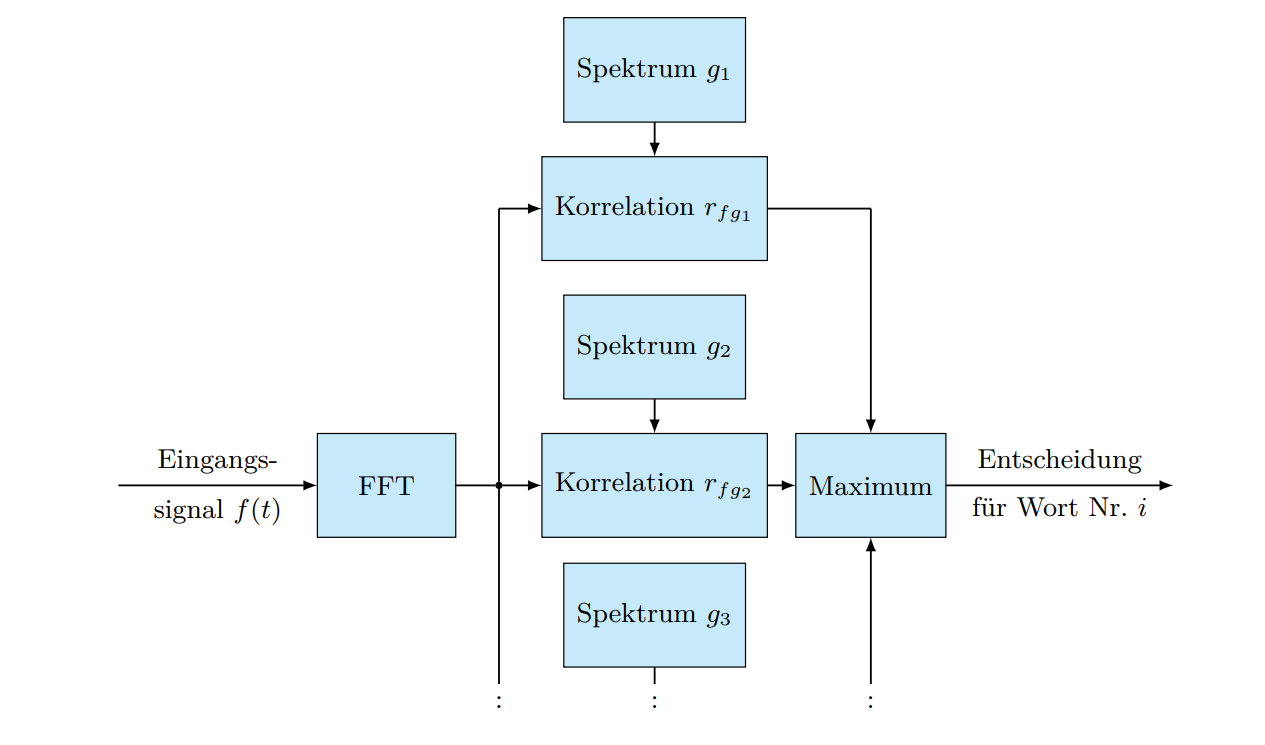
\includegraphics[width=.9\linewidth]{media/archi.png}
	\caption{Architektur des Spracherkenners}
	\label{img:Architektur des Spracherkenners}
\end{figure}
%
% CHAPTER Versuch 1
%
\chapter{Versuch 1}
\label{chap:VERSUCH_1}

\section{Fragestellung, Messprinzip, Aufbau, Messmittel}
\label{chap:VERSUCH_1_FRAGESTELLUNG}

\textbf{Fragestellung:}
\newline
In dem ersten Teil des Versuchs \textit{'Aufbau eines einfachen Spracherkenners'} werden wir einen Spracherkenner bauen.
Zudem erweitern wir den Spracherkenner mit einer Triggerfunktion.
Mit der Aufnahme bestimmen wir dessen Amplitudenspektrum.
Im Anschluss werden die Methode des Windowing anwenden.
\newline
So werden wir eine Testaufnahme machen um diese anschließend auszuwerten. 
\newline
Auf die entstandenen Numpy-Dateien wenden wir Windowing und das Amplitudenspektrum an.
\newline
\newline
\textbf{Messprinzip:}
\newline
Im ersten Versuch starten wir mit einem Pythonskript. Das Mikrofon wird mit einem Klinkenstecker direkt an die Soundkarte des Computers verbunden.
Auf den Computern im Labor, ist das Paket PyAudio bereits in den IDE's integriert.
\newline
Mit dem geschriebenen Pythonskript können wir nun akustische Signale aufnehmen. 
Über das Objekt \textit{audiorecorder} haben wir Zugriff auf die Aufnahmefunktion der Soundkarte.
\newline
Das Signal speichern wir anschließend mittels \textit{numpy.save()}.
Im Anschluss sollen wir eine beliebige Spracheingabe aufnehmen und diese in einem Diagramm darstellen.
\newline
\newline
Im Anschluss sollen wir das Aufnahmeprogramm um eine Triggerfunktion erweitern, welche die Aufnahme erst ab einem gewissen Lautstärkepegel starten lässt.
\newline
So können wir sicher stellen, dass alle Aufnahmen den selben Startpunkt besitzen.
\newpage
Das Signal soll eine Dauer von einer Sekunde haben und die fehlenden Samples mit Nullen augefüllt werden.
\newline
\newline
Mit dem Code Aus dem dritten Versuch können wir mit der Aufnahme das Amplitudenspektrum bestimmen.
Dies stellen wir grapisch dar.
Danach implementieren die Methode des Windowing. 
\newline
Diese werden wir jeweils in einer Länge von 512 Samples darstellen.
Die einzelnen Windows werden wir mit der Gaußschen Fensterfunktion multiplizieren  die eine Fensterbreite von der Standartabweichung 4 hat.
\newline
Den ersten Versuch werden wir mit dem Amplitudenspektrum erneut überprüfen und so das Spektrum aus der letzten Aufgabe auf Korrektheit überprüfen.
\newline
\newline
\textbf{Aufbau:}
\newline
Das Mikrofon wird durch einen Klinkenstecker direkt an die Soundkarte des Computers verbunden.
Durch ein Pythonskript können wir nun Sprachaufnahmen machen.
\begin{figure}[H]
	\centering
	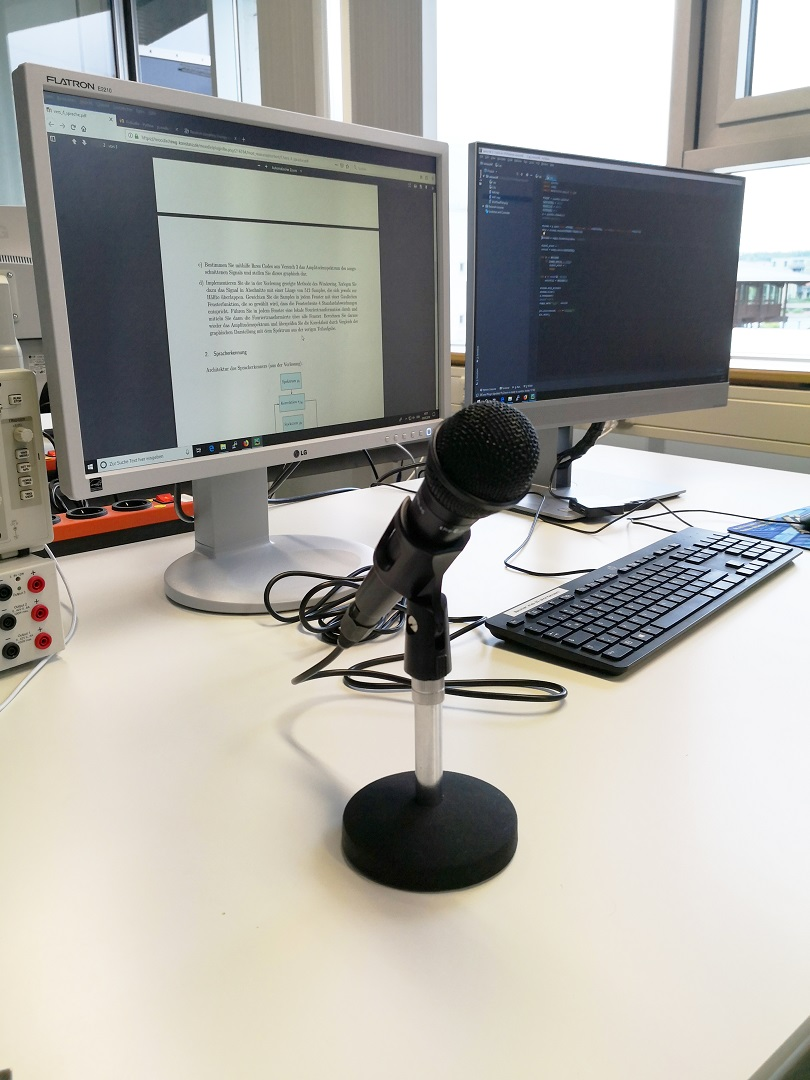
\includegraphics[width=.5\linewidth]{media/aufbau.jpg}
	\caption{Aufnahme mit Triggerfunktion des Wortes rechts}
	\label{img:Aufnahme mit Triggerfunktion des Wortes rechts}
\end{figure}
\newpage
\textbf{Messmittel:}
\item[NichtnummerierteAufzahlung]~\par
   \begin{itemize}
      \item Ein Mikrofon
      \item Ein Computer mit einer Python IDE
   \end{itemize}
\newpage
\section{Messwerte}
\label{chap:VERSUCH_1_MESSWERTE}
Mit einem Mikrofon das an den Computer angeschlossen ist, sehen wir die mit dem Pythonskript aufgenommene Sprachaufnahme des Wortes \textit{'Test'}, welche mit Python visualisiert wurde.
\newline
In der linken Darstellung ist die gesamte Dauer des empfangenen Signals, welche sich durch einen einfachen Plot des Signals darstellen lässt.
\newline
Im rechten Bild ist eine verkürzte Darstellung der Sprachaufnahme um das Signal besser zu erkennen welches durch \textit{plt.xlim(0, 35000)} auf eine Frequenz von 35000 limitiert wird.

\begin{figure}[hbt!]
\centering
	\begin{subfigure}{.5\textwidth}
  		\centering
 		 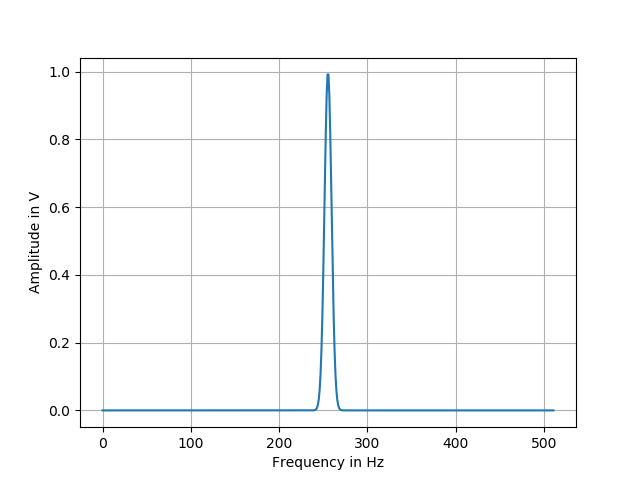
\includegraphics[width=.95\linewidth]{../data/img/testamp.png}
  		\caption{Sprachaufnahme des Wortes Test}
 		 \label{fig:sub1}
	\end{subfigure}%
	\begin{subfigure}{.5\textwidth}
  		\centering
 		 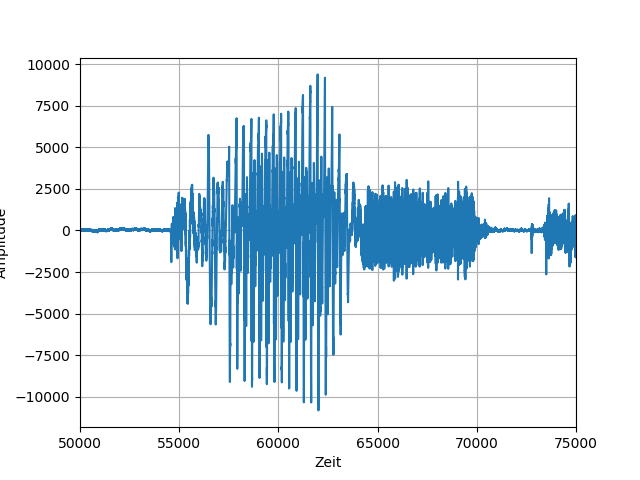
\includegraphics[width=.95\linewidth]{../data/img/testamp2.png}
  		\caption{Dieselbe Sprachaufnahme mit kurzer Zeitachse}
  		\label{fig:sub2}
	\end{subfigure}
	\caption{Die aufgenommene Sprachaufnahme visualisiert mit Python}
	\label{fig:test}
\end{figure}
Die Aufnahme wurde durch die Funktion \textit{p.open()} gestartet. 
\newline
Im Gegensatz zum zweiten Teil der Aufgabe wird hier bereits durch das Starten des Skriptes aufgenommen.
\newpage
Im folgenden sieht man die Sprachaufnahme des Wortes 'Rechts' mit der Triggerfunktion.
Die Aufnahme läuft bereits durch das Starten des Programmes.
\newline
Die Stelle bei der die Überschreitung des Schwellenwertes geschieht wird gespeichert und beginnt ab dieser Stelle.
\newline
Durch die Triggerfunktion startet die Aufnahme dadurch erst ab dem Schwellenwert.
\begin{figure}[H]
	\centering
	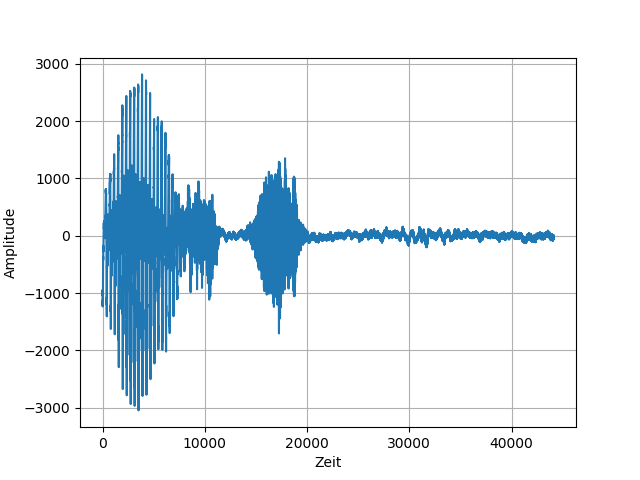
\includegraphics[width=.75\linewidth]{../data/img/rechtsamp.png}
	\caption{Aufnahme mit Triggerfunktion des Wortes rechts}
	\label{img:Aufnahme mit Triggerfunktion des Wortes rechts}
\end{figure}

\newpage
\section{Auswertung}
\label{chap:VERSUCH_1_AUSWERTUNG}
Auf der linken Seite ist das Amplitudenspektrum und auf der rechten Seite das Amplitudenspektrum bis zur Frequenz von 1000.
\newline
Diese wurden mit der Formel berechnet. Mit der Anwendung der Formel auf jedes eingegangene Signal erhalten wir den folgenden Plot:

\begin{figure}[H]
\centering
	\begin{subfigure}{.5\textwidth}
  		\centering
 		 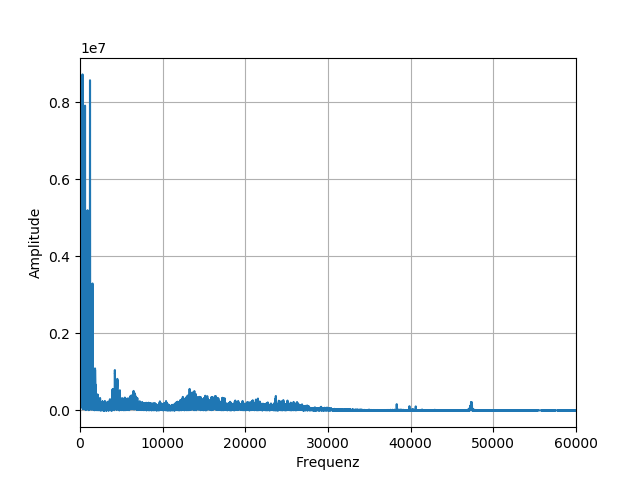
\includegraphics[width=.95\linewidth]{../data/img/testspektrum1.png}
  		\caption{Amplitudenspektrum der Sprachaufnahme}
 		 \label{fig:sub1}
	\end{subfigure}%
	\begin{subfigure}{.5\textwidth}
  		\centering
 		 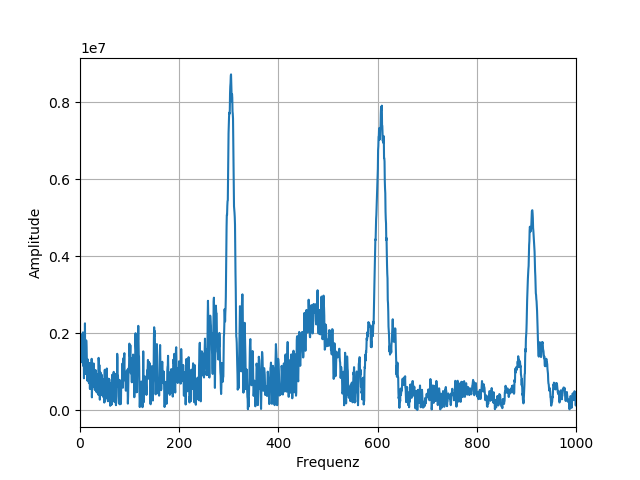
\includegraphics[width=.95\linewidth]{../data/img/testspektrum3.png}
  		\caption{Amplitudenspektrum mit geringerer Frequenz}
  		\label{fig:sub2}
	\end{subfigure}
	\caption{Das Amplitudenspektrum mit der dazugehörigen Frequenz}
	\label{fig:test}
\end{figure}
\newline
Im folgenden sieht man eine Gaußsche Fensterfunktion mit der Fensterbreite von 4 Standardabweichungen.
\begin{figure}[H]
	\centering
	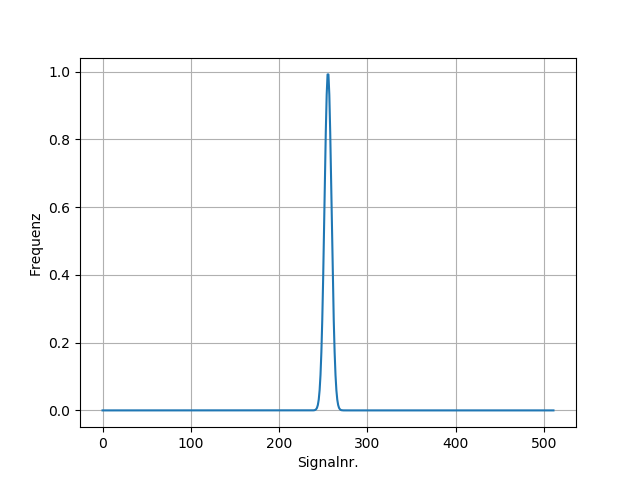
\includegraphics[width=.7\linewidth]{../data/img/gauss.png}
	\caption{Gausssche Fensterfunktion mit Standardabweichung 4}
	\label{img:Gausssche Fensterfunktion mit Standardabweichung 4}
\end{figure}
Im Anschluss zerlegt man das Signal in Abschnitte mit der von Länge 512 Samples, die sich jeweils zur Hälfte überlappen sollen.
Das Signal wird mit dem entsprechenden Signal der Gaußschen Fensterfunktion multipliziert und daraufhin eine lokale Fouriertransformation durchgeführt.
Zu guter Letzt werden die Fouriertransformierten über alle Fenster gemittelt.

\begin{figure}[H]
	\centering
	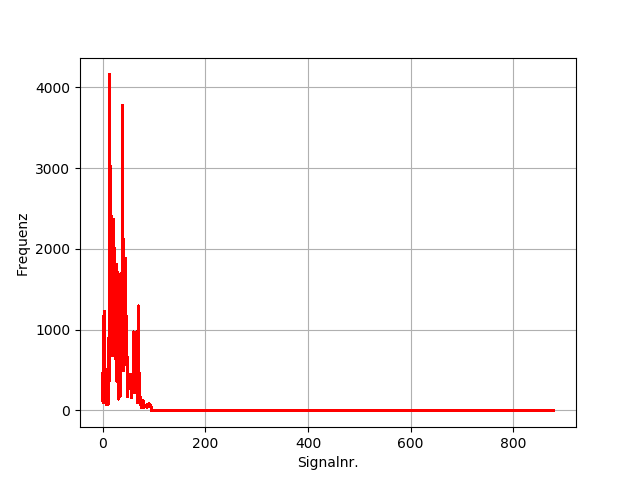
\includegraphics[width=.6\linewidth]{../data/img/AlleRichtig.png}
	\caption{Aufnahme mit Triggerfunktion des Wortes rechts}
	\label{img:Aufnahme mit Triggerfunktion des Wortes rechts}
\end{figure}
Das Windowing wird auf das Signal angewandt. Nachdem zum Beispiel bei dem Wort 'Hoch' über 170 Windows ausgegeben wurden als Plot, sieht der Explorer folgendermaßen aus.
\begin{figure}[H]
	\centering
	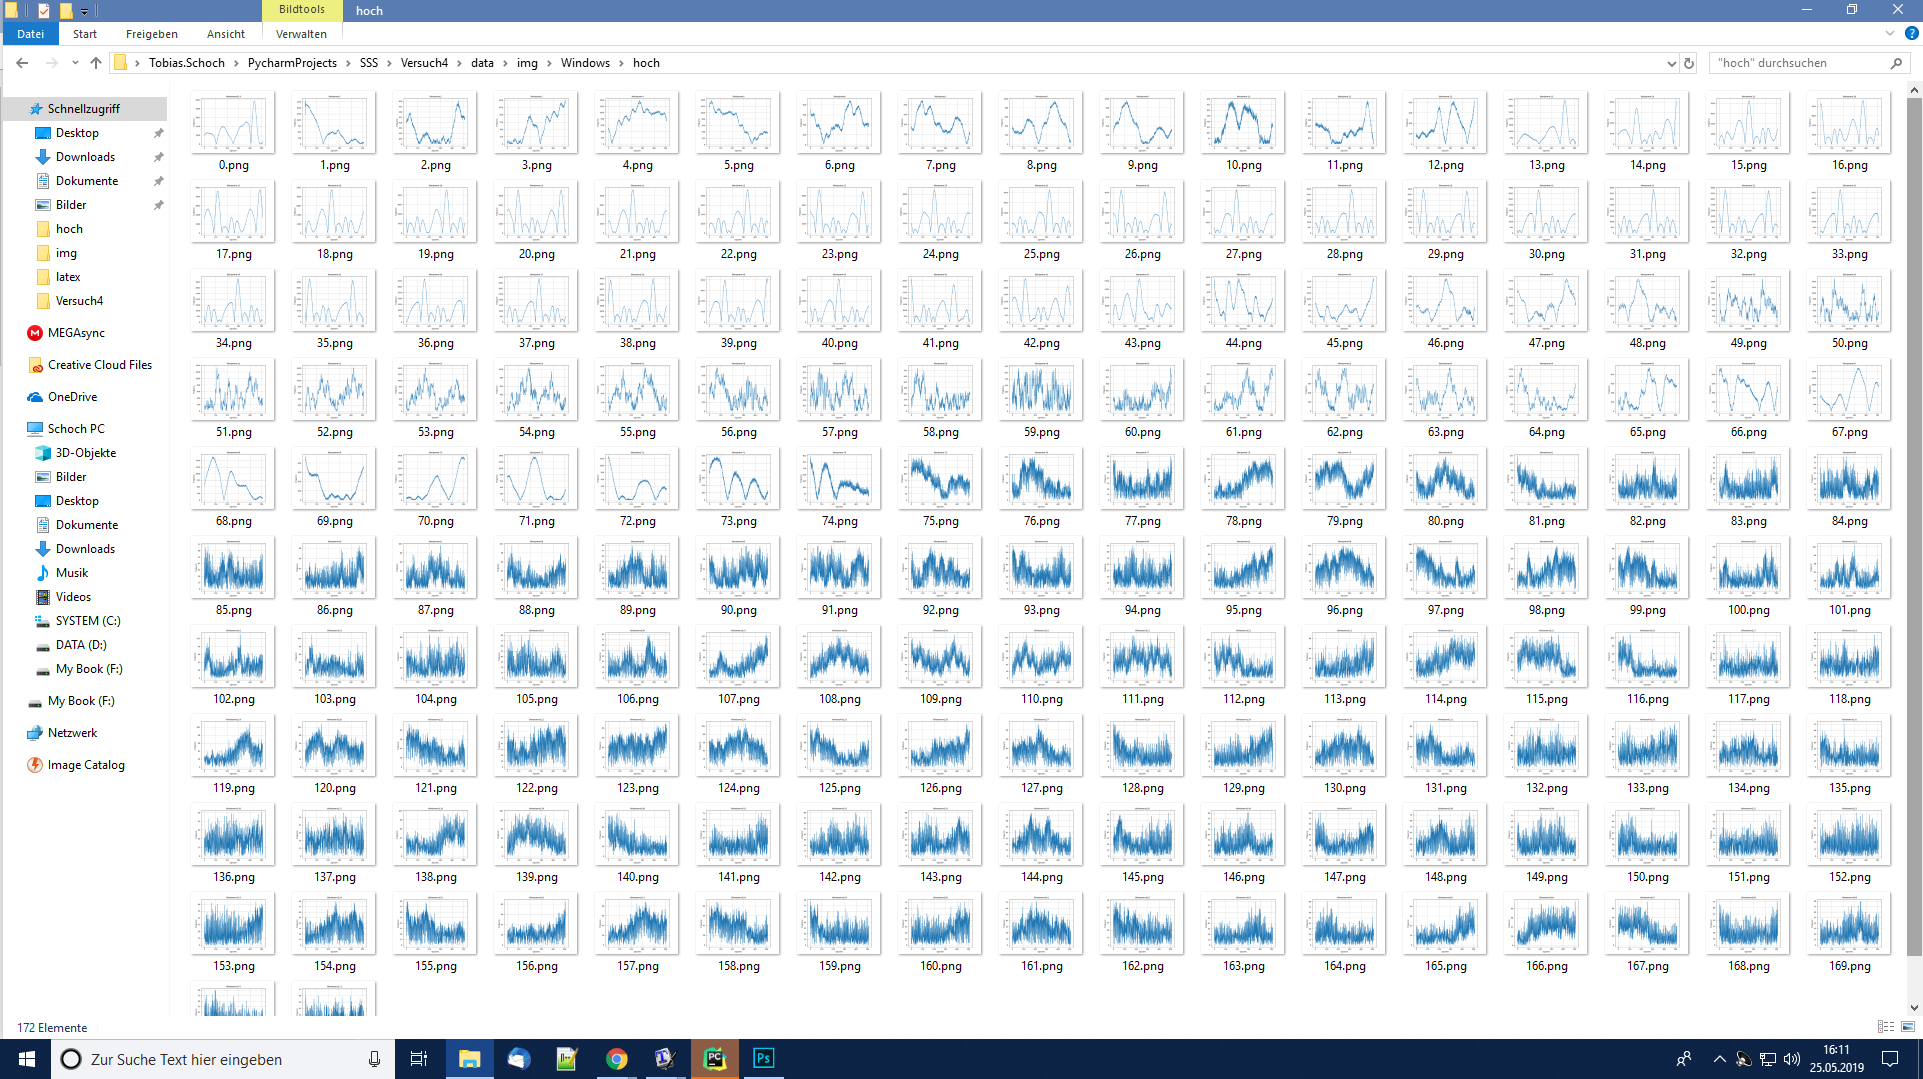
\includegraphics[width=.8\linewidth]{../data/img/window.png}
	\caption{Aufnahme mit Triggerfunktion des Wortes rechts}
	\label{img:Aufnahme mit Triggerfunktion des Wortes rechts}
\end{figure}
\newpage
\section{Interpretation}
\label{chap:VERSUCH_1_INTERPRETATION}
Bei der Betrachtung der Sprachaufnahme sehen wir die übliche Amplituden und Frequenzen bei der Aussprache des Wortes 'Test'.
In der Vergrößerung sind nochmals besser die Amplitudenausschläge zu sehen.
\newline 
\newline
In der Abbildung 2.3 sieht man die Sprachaufnahme des Wortes 'Rechts'.
Die Aufnahme wurde mit einem Pythonskript gemacht, dass eine Triggerfunktion implementiert hat.
Ab einem bestimmten Schwellenwert beginnt die Aufnahme. Hier ist es schön zu sehen, dass die Aufnahme nicht mit Start des Skriptes beginnt, sondern erst wenn gesprochen wird. 
\newline 
\newline
Auf das Signal wurde daraufhin das Amplitudenspektrum berechnet. Durch dieses erfährt man die Frequenzen die in einem Wort stecken.
Der größte Ausschlag bei der Frequenz mit eienr Amplitude von über 0.8 ist die maximalste Amplitude. Die Frequenz liegt bei knapp über 300Hz.
Die x Achse wurde  auf die Hälfte gekürzt, da bei ein Amplitudenspektrum sich nach der Hälfte wiederholt.
\newline
\newline
Wenn man diese mit dem Gaußschen Fenster multipliziert, erhält man die gemittelten fouriertransfomierten Fenster.
Desto höher der absolute Ausschlag, desto höher ist die Amplitude im Window. Durch den senkrechten Ausschnitte sind steile Übergänge erzeugt
worden, die im ursprünglichen Signal nicht vorhanden sind. 
Steile Übergänge erzeugen jedoch viele hohe Frequenzen im Spektrum.
%
% CHAPTER Versuch 2
%
\chapter{Versuch 2}
\label{chap:VERSUCH_2}
\section{Fragestellung, Messprinzip, Aufbau, Messmittel}
\label{chap:VERSUCH_2_FRAGESTELLUNG}
Im zweiten Versuch müssen wir vier verschiedene Befehle jeweils fünf mal aufnehmen. 
\newline
Die Befehle die wir aufnehmen lauten:
\item[NichtnummerierteAufzahlung]~\par
   \begin{itemize}
      \item Links
      \item Rechts
      \item Hoch
      \item Tief
   \end{itemize}
Anhand der aufgenommenen Numpy Funktionen berechnen wir die Spektren mit der Windowing Methode.
Daraufhin berechnen wir noch die eigentlichen Referenzspektren.
\newline
Im Anschluss berechnen wir noch den Korrelationskoeffizienten nach Bravais-Pearson mit dem wir zwei verschiedene Spektren miteinander vergleichen können.
\newline
Dafür brauchen wir vom selben und einem anderen Sprecher erneut Sprachaufnahmen.
\newline
Mit diesen testen wir die Routine an den Referenzspektren: 
\newline
Beim Vergleich identischer Spektren sollte die Korrelation 1 sein, bei verschiedenen Spektren nahe an 0.
\newline
Zudem sollen wir eine Fehler- und eine Detektionsrate angeben.

\section{Messwerte}
\label{chap:VERSUCH_2_MESSWERTE}
Die sämtlichen aufgenommenen Sprachaufnahmen in Form von Numpy-Dateien werden wir mit der Windowing Methode in Spektren berechnen.
Dabei wird erstmal das Spektrum mit der Gaußschen Fensterfunktion berechnet und multipliziert mit den einzelnen Windows.
\newline
Danach wird das Fenster absolut fouriertransformiert.
Daraus wiederrum wird der Durchschnitt berechnet. 
\begin{figure}[H]
	\centering
	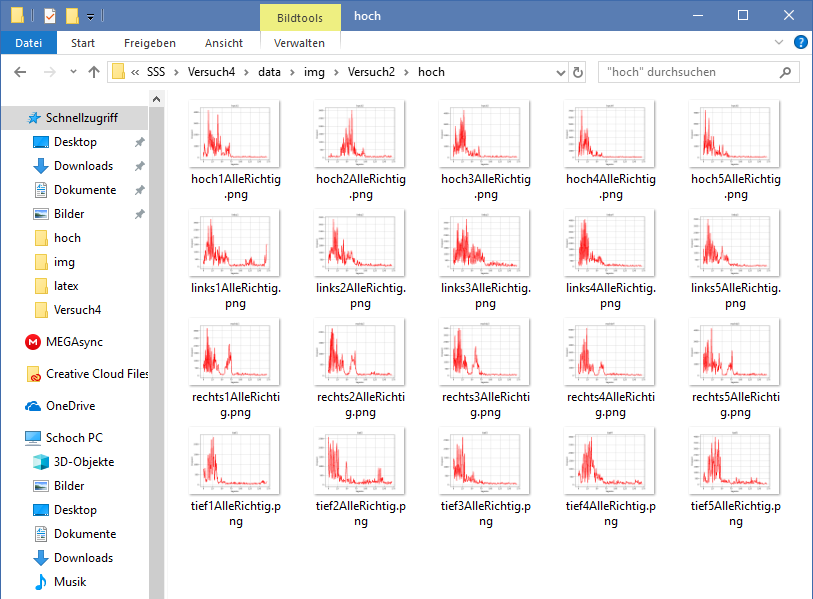
\includegraphics[width=.7\linewidth]{media/folder.png}
	\caption{Sämtliche Signale mit Windowing berechnet}
	\label{img:Sämtliche Signale mit Windowing berechnet}
\end{figure}

\begin{figure}[H]
\centering
	\begin{subfigure}{.5\textwidth}
  		\centering
 		 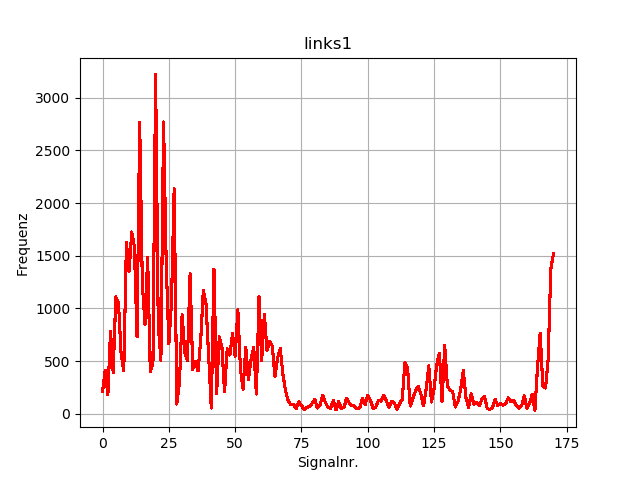
\includegraphics[width=.95\linewidth]{../data/img/Versuch2/hoch/links1AlleRichtig.png}
  		\caption{Erste Sprachaufnahme von 'links'}
 		 \label{fig:sub1}
	\end{subfigure}%
	\begin{subfigure}{.5\textwidth}
  		\centering
 		 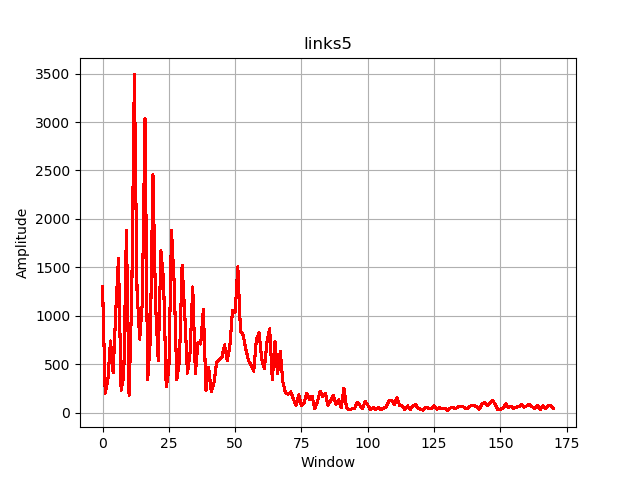
\includegraphics[width=.95\linewidth]{../data/img/Versuch2/hoch/links5AlleRichtig.png}
  		\caption{Fünfte Sprachaufnahme von 'links'}
  		\label{fig:sub2}
	\end{subfigure}
	\caption{Zwei verschiedene Sprachaufnahmen im Vergleich.}
	\label{fig:test}
\end{figure}
\newpage
\section{Auswertung}
\label{chap:VERSUCH_2_AUSWERTUNG}
Die Daten aus den Numpydateien werden in einzelne Windows zerlegt mit einer Länge von 512 Samples die sich jeweils überlappen.
\newline
Die einzelnen Samples werden mit der Gaußschen Fensterfunktion multipliziert, welche eine Fensterbreite von 4 Standardabweichungen hat.
In jedem Fenster wird eine lokale Fouriertransformation durchgeführt.
Daraufhin werden die Fouriertransformierten über alle Fenster gemittelt.
\newline
Nachdem man sämtliche 4 Befehle und die jeweils fünf Beispiel dazu gemittelt hat, erhält man das Referenzspektrum.
\begin{figure}[H]
\centering
	\begin{subfigure}{.5\textwidth}
  		\centering
 		 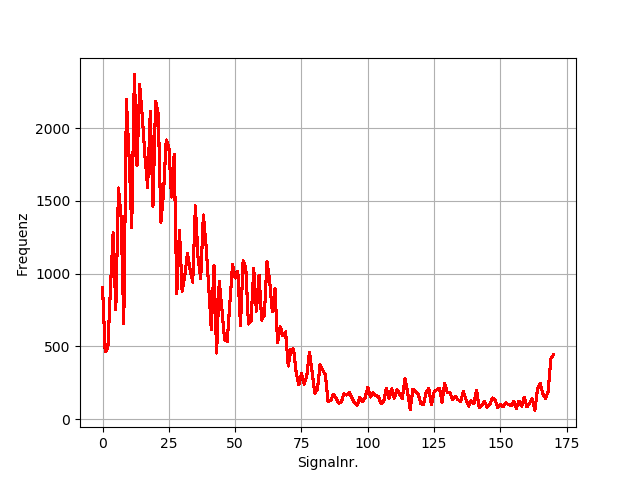
\includegraphics[width=.95\linewidth]{../data/img/Versuch2/2Averagelinks.png}
  		\caption{Person 1: Referenzspektrum 'Links'}
 		 \label{fig:sub1}
	\end{subfigure}%
	\begin{subfigure}{.5\textwidth}
  		\centering
 		 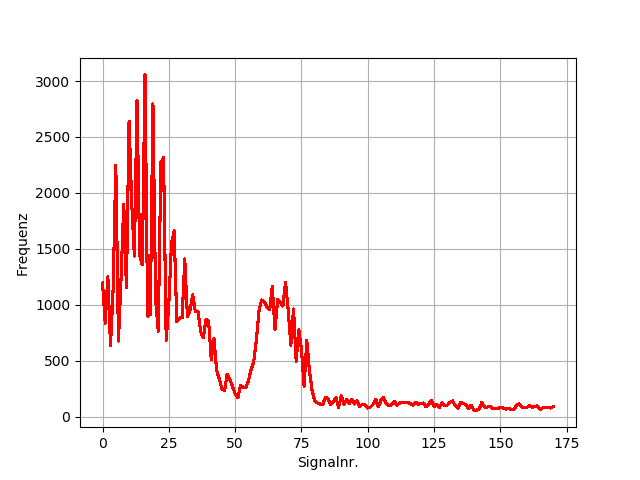
\includegraphics[width=.95\linewidth]{../data/img/Versuch2/2Averagerechts.png}
  		\caption{Person 1: Referenzspektrum 'Rechts'}
  		\label{fig:sub2}
	\end{subfigure}
\begin{subfigure}{.5\textwidth}
  		\centering
 		 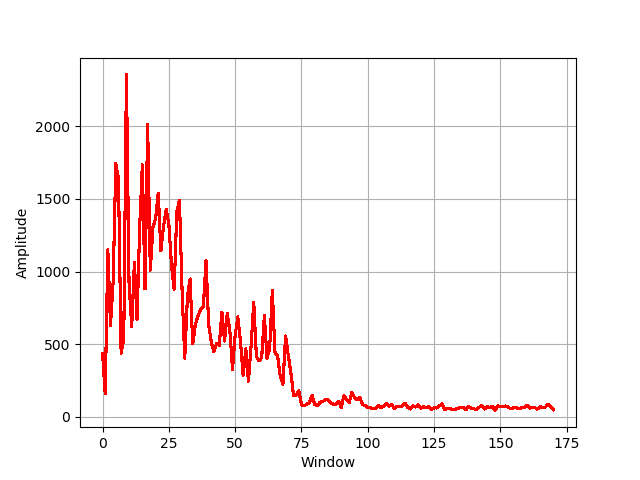
\includegraphics[width=.95\linewidth]{../data/img/Versuch2/2Averagehoch.png}
  		\caption{Person 1: Referenzspektrum 'Hoch'}
 		 \label{fig:sub3}
	\end{subfigure}%
	\begin{subfigure}{.5\textwidth}
  		\centering
 		 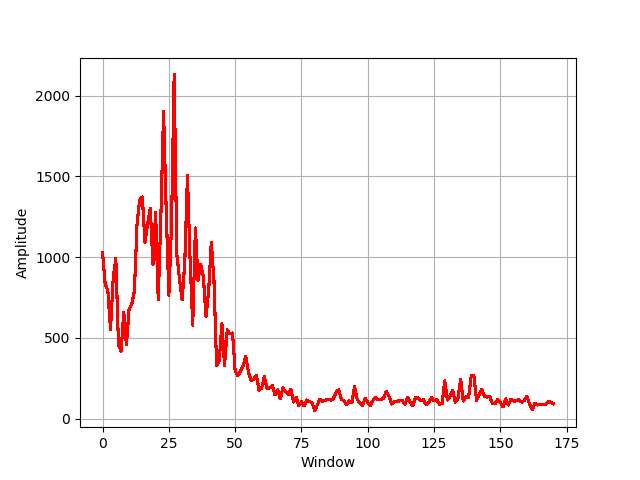
\includegraphics[width=.95\linewidth]{../data/img/Versuch2/2Averagetief.png}
  		\caption{Person 1: Referenzspektrum 'Tief'}
  		\label{fig:sub4}
	\end{subfigure}
	\caption{Die vier Referenzspektren}
	\label{fig:2test}
\end{figure}
\newpage
Hier werden zwei Eingabespektren beziehungsweise zwei Dateien mittels der Bravais-Pearson Methode verglichen auf ihre Korrelationskoeffizienten.
\newline
Wenn die Spektren identisch sind, sollte der Wert 1.0 ergeben. Bei ungleichen Spektren sollte dieser nahe 0 sein.
Person 1 ist die Person, welche die Spracheeingabe gemacht hat.

\begin{table}[H]
	\centering\small
	\begin{tabular}{||c | c | c||}
		 \hline
		 Spracheingabe & Person 1 & Person 2 \\ [0.5ex] 
		 \hline
		 \textbf{Hoch} & \textbf{0.5817} & \textbf{0.5496} \\ 
		 \hline
		 1 - Hoch & 0.6856 & 0.6283 \\ 
		 \hline
		 2 - Hoch & 0.5001 & 0.6000 \\ 
		 \hline
		 3 - Hoch & 0.5829 & 0.5600 \\ 
		 \hline
		 4 - Hoch & 0.5754 & 0.4902 \\ 
		 \hline
		 5 - Hoch & 0.5644 & 0.4691 \\ 
		 \hline
		 \textbf{Tief} & \textbf{0.7088} & \textbf{0.6172} \\
		 \hline
		 1 - Tief & 0.6682 & 0.5976 \\ 
		 \hline
		 2 - Tief & 0.7210 & 0.6520 \\ 
		 \hline
		 3 - Tief & 0.6947 &0.4947 \\ 
		 \hline
		 4 - Tief & 0.7069 &0.6098 \\ 
		 \hline
		 5 - Tief & 0.7531 & 0.7318 \\ 
		\hline
		\textbf{Links} & \textbf{0.6514} & \textbf{0.6084} \\
		\hline
		 1 - Links & 0.6708 & 0.5711 \\ 
		 \hline
		 2 - Links & 0.6451 & 0.5953 \\ 
		 \hline
		 3 - Links & 0.6273 & 0.5785 \\ 
		 \hline
		 4 - Links & 0.6472 & 0.6512 \\ 
		 \hline
		 5 - Links & 0.6666 &  0.6460 \\ 
		 \hline
		 \textbf{Rechts} & \textbf{0.4219} & \textbf{0.1779} \\
		 \hline
		 1 - Rechts & 0.5001 & 0.1401 \\ 
		 \hline
		 2 - Rechts & 0.5402 & 0.2892 \\ 
		 \hline
		 3 - Rechts & 0.5032 & 0.2790 \\ 
		 \hline
		 4 - Rechts & 0.3895 & 0.2849 \\ 
		 \hline
		 5 - Rechts & 0.1764 & 0.1764 \\ 
		 \hline
	\end{tabular}
	\caption{Vergleich der berechneten Referenzspektren}
	\label{fig:Vergleich der berechneten Referenzspektren}
\end{table}
\newpage

\begin{figure}[H]
\centering
	\begin{subfigure}{.5\textwidth}
  		\centering
 		 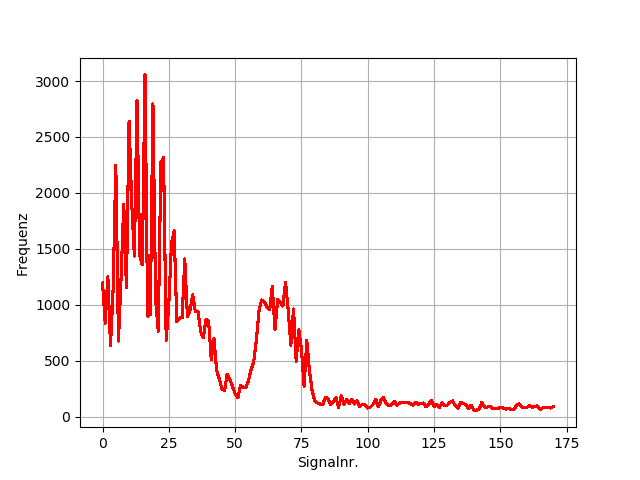
\includegraphics[width=.95\linewidth]{../data/img/Versuch2/2Averagerechts.png}
  		\caption{Person 1: Referenzspektrum 'Rechts'}
 		 \label{fig:sub1}
	\end{subfigure}%
	\begin{subfigure}{.5\textwidth}
  		\centering
 		 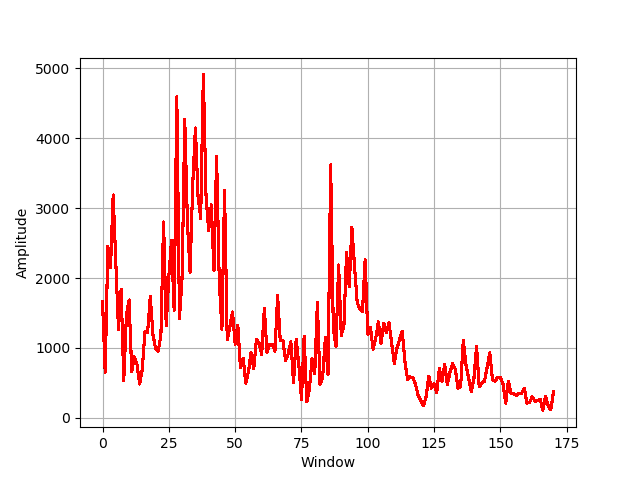
\includegraphics[width=.95\linewidth]{../data/img/Versuch2/Averagerechts.png}
  		\caption{Person 2: Referenzspektrum 'Rechts'}
  		\label{fig:sub2}
	\end{subfigure}
\begin{subfigure}{.5\textwidth}
  		\centering
 		 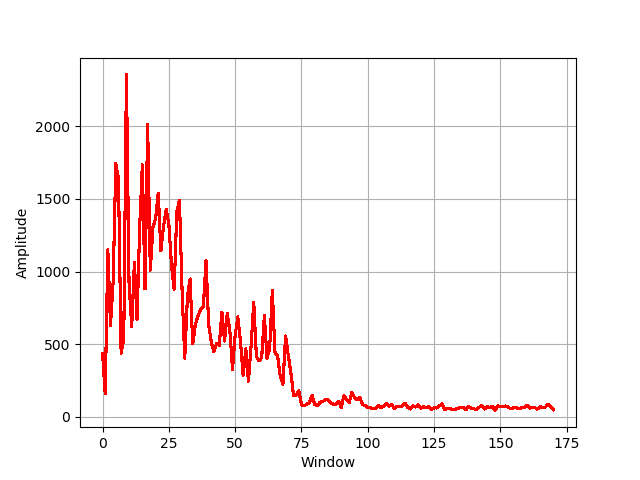
\includegraphics[width=.95\linewidth]{../data/img/Versuch2/2Averagehoch.png}
  		\caption{Person 1: Referenzspektrum 'Hoch'}
 		 \label{fig:sub3}
	\end{subfigure}%
	\begin{subfigure}{.5\textwidth}
  		\centering
 		 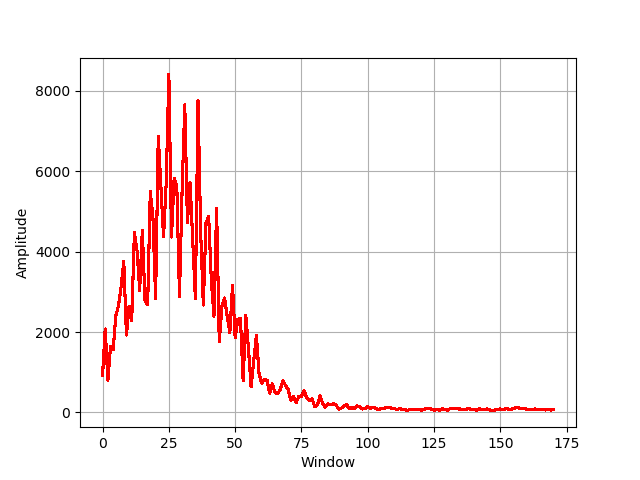
\includegraphics[width=.95\linewidth]{../data/img/Versuch2/Averagehoch.png}
  		\caption{ Person 2: Referenzspektrum 'Hoch'}
  		\label{fig:sub4}
	\end{subfigure}
	\caption{Die vier Referenzspektren mit den größten Unterschieden}
	\label{fig:test2}
\end{figure}
\newpage
\section{Interpretation}
\label{chap:VERSUCH_2_INTERPRETATION}
In Abbildung [\ref{fig:test}] sieht man, wie sich Sprachaufnahmen von der selben Person mit dem selben Wort unterscheiden können.
Im hinteren Teil von der linken Abbildung sieht man zum Schluß eine Steigung der Spannung. 
\newline
Diese ist entstanden durch ungefähr 8 bis 9 andere Gruppen im Raum, durch welche die Hintergrundgeräusche sehr laut waren.
Die anderen Geräusche unterscheiden sich nur geringfügig.
\newline
\newline
Nachdem wir die Signale ausgewertet haben, haben wir mit der Windowing Methode und der Bravais-Pearson den Korrelationskoeffizienten berechnet.
In der Abbildung [\ref{fig:2test}] sieht man die durchschnittlichen Spektren für eines der Worte (Hoch, Tief, Links, Rechts).
\newline
Dabei ähneln sich die Spektren der Wiederholungen der Worte sehr. Das Wort rechts hat ein sehr ausgeprägtes Spektrum. 
\newline
Am Anfang geht das Signal sehr steil nach oben durch das Vokal 'e'.
Bei den Konsonanten 'ch' gibt es eine sehr große Verringerung. Zum Schluss bei 's' geht das Signal wieder nach oben.
So kann man gut die einzelnen Buchstaben des Wortes identifizieren.
\newline
\newline
Bei der Bravais-Pearson Methode mit den Referenzspektren und der erneuten Aufnahme der Worte erhält man eine Lange Tabelle mit einigen Werten.
Am deutlichsten ist der Unterschied bei der Aufnahme mit dem Wort 'Rechts'.
\newline
Auch ist es gut sichtbar bei einzelnen Aufnahmen mit dem Wort 'Tief'.
Der größte Unterschied liegt bei 0.35, was ziemlich viel ist, wenn man die Skala von 1.0 - 0.0 betrachtet.
\newline
Die Bravais-Pearson Korrelationskoeffizientenberechnung hat sich gelohnt und als richtig erwiesen, da die Werte immer bei den Sprachaufnahmen der selben Person höher waren, als bei der fremden Person.
\newline
\newline
Hier [\ref{fig:test2}] kann nochmal gut einzelne Spektren begutachten, die das selbe Wort von unterschiedlichen Menschen darstellen.
Man kann gut betrachten, dass der zweite Sprecher definitiv energischer und lauter gesprochen hat.
\newline
Die Amplituden liegen im zwei- bis sogar dreifachen Bereich und haben ein sehr viel unruhigeres Spektrum.

%
% CHAPTER Anhang
%
\renewcommand\thesection{A.\arabic{section}}
\renewcommand\thesubsection{\thesection.\arabic{subsection}}

\chapter*{Anhang}
\label{chap:APPENDIX}
\addcontentsline{toc}{chapter}{Anhang}
%\setcounter{chapter}{0}
\addtocounter{chapter}{1}
\setcounter{section}{0}

\section{Quellcode}
\label{chap:APPENDIX_SOURCECODE}

\subsection{Quellcode Versuch 1}
\label{chap:APPENDIX_SOURCECODE_V1}
\lstinputlisting[style=PYTHON, frame=single, caption=Einlesen der Sprachaufnahme und ablegen des Signals in eine Numpy Datei, captionpos=b, label=lst:APPENDIX_SOURCECODE_AREA1]{../task1.1.py}
\newpage
\lstinputlisting[style=PYTHON, frame=single, caption=Einlesen einer Sprachaufnahme mit Aktivierung durch Triggerung, captionpos=b, label=lst:APPENDIX_SOURCECODE_AREA2]{../task1.2.py}
\newpage
\lstinputlisting[style=PYTHON, frame=single, caption=Amplitudenspektrum und Ausgabe von Plots, captionpos=b, label=lst:APPENDIX_SOURCECODE_AREA3]{../task1.3.py}
\newpage
\lstinputlisting[style=PYTHON, frame=single, caption=Windowing und Ausgabe von Plots bzw. Windows, captionpos=b, label=lst:APPENDIX_SOURCECODE_AREA4]{../task1.4.py}
\newpage
\subsection{Quellcode Versuch 2}
\label{chap:APPENDIX_SOURCECODE_V2}
\lstinputlisting[style=PYTHON, frame=single, caption=Windowing und Mittelung der Spektren, captionpos=b, label=lst:APPENDIX_SOURCECODE_AREA5]{../task2.1.py}
\newpage
\lstinputlisting[style=PYTHON, frame=single, caption=Windowing und Bravais-Pearson Methode, captionpos=b, label=lst:APPENDIX_SOURCECODE_AREA6]{../task2.2.py}
\lstinputlisting[style=PYTHON, frame=single, caption=Bravais-Pearson Methode mit Ausgabe der Korrelation, captionpos=b, label=lst:APPENDIX_SOURCECODE_AREA7]{../task2.3.py}

%
% Literaturverzeichnis
%
%
% Literaturverzeichnis
%
\phantomsection
\addcontentsline{toc}{chapter}{Literaturverzeichnis}
\bibliography{../references}
\newpage

\end{document}
%------------------------------------
% ╔═╗╔╗╔╔╦╗  ╔╦╗╔═╗╔═╗╦ ╦╔╦╗╔═╗╔╗╔╔╦╗
% ║╣ ║║║ ║║   ║║║ ║║  ║ ║║║║║╣ ║║║ ║ 
% ╚═╝╝╚╝═╩╝  ═╩╝╚═╝╚═╝╚═╝╩ ╩╚═╝╝╚╝ ╩ 
%------------------------------------